\documentclass[10pt,dvipdfmx]{jsarticle}
\usepackage{graphicx}
\usepackage{titlesec}
\usepackage{amssymb}
\titleformat*{\section}{\normalsize\bfseries}
\titleformat*{\subsection}{\normalsize\bfseries}

\usepackage{tikz}
\usetikzlibrary{matrix,calc}

%internal group
%#1-space between node and grouping line. Default=0
%#2-top left node
%#3-bottom right node
\newcommand{\implicant}[3][0]{
    \draw[rounded corners=3pt] ($(#2.north west)+(135:#1)$) rectangle ($(#3.south east)+(-45:#1)$);
    }

%group lateral borders
%#1-space between node and grouping line. Default=0
%#2-top left node
%#3-bottom right node
\newcommand{\implicantcostats}[3][0]{
    \draw[rounded corners=3pt] ($(rf.east |- #2.north)+(90:#1)$)-| ($(#2.east)+(0:#1)$) |- ($(rf.east |- #3.south)+(-90:#1)$);
    \draw[rounded corners=3pt] ($(cf.west |- #2.north)+(90:#1)$) -| ($(#3.west)+(180:#1)$) |- ($(cf.west |- #3.south)+(-90:#1)$);
}

%group top-bottom borders
%#1-space between node and grouping line. Default=0
%#2-top left node
%#3-bottom right node
\newcommand{\implicantdaltbaix}[3][0]{
    \draw[rounded corners=3pt] ($(cf.south -| #2.west)+(180:#1)$) |- ($(#2.south)+(-90:#1)$) -| ($(cf.south -| #3.east)+(0:#1)$);
    \draw[rounded corners=3pt] ($(rf.north -| #2.west)+(180:#1)$) |- ($(#3.north)+(90:#1)$) -| ($(rf.north -| #3.east)+(0:#1)$);
}

%group corners
%#1-space between node and grouping line. Default=0
\newcommand{\implicantcantons}[1][0]{
    \draw[rounded corners=3pt] ($(rf.east |- 0.south)+(-90:#1)$) -| ($(0.east |- cf.south)+(0:#1)$);
    \draw[rounded corners=3pt] ($(rf.east |- 8.north)+(90:#1)$) -| ($(8.east |- rf.north)+(0:#1)$);
    \draw[rounded corners=3pt] ($(cf.west |- 2.south)+(-90:#1)$) -| ($(2.west |- cf.south)+(180:#1)$);
    \draw[rounded corners=3pt] ($(cf.west |- 10.north)+(90:#1)$) -| ($(10.west |- rf.north)+(180:#1)$);
}

%Empty Karnaugh map 4x4
\newenvironment{Karnaugh}%
{
\begin{tikzpicture}[baseline=(current bounding box.north),scale=0.8]
\draw (0,0) grid (4,4);
\scriptsize \draw (0,4) -- node [pos=1,right,anchor=south west] {$x_2 x_1$} node [pos=0.7,below left,anchor=north east] {$\tiny x_4 x_3$} ++(135:1);
%
\normalsize \matrix (mapa) [matrix of nodes,
        column sep={0.8cm,between origins},
        row sep={0.8cm,between origins},
        every node/.style={minimum size=0.3mm},
        anchor=8.center,
        ampersand replacement=\&] at (0.5,0.5)
{
                       \& |(c00)| 00         \& |(c01)| 01         \& |(c11)| 11         \& |(c10)| 10         \& |(cf)| \phantom{00} \\
|(r00)| 00             \& |(0)|  \phantom{0} \& |(1)|  \phantom{0} \& |(3)|  \phantom{0} \& |(2)|  \phantom{0} \&                     \\
|(r01)| 01             \& |(4)|  \phantom{0} \& |(5)|  \phantom{0} \& |(7)|  \phantom{0} \& |(6)|  \phantom{0} \&                     \\
|(r11)| 11             \& |(12)| \phantom{0} \& |(13)| \phantom{0} \& |(15)| \phantom{0} \& |(14)| \phantom{0} \&                     \\
|(r10)| 10             \& |(8)|  \phantom{0} \& |(9)|  \phantom{0} \& |(11)| \phantom{0} \& |(10)| \phantom{0} \&                     \\
|(rf) | \phantom{00}   \&                    \&                    \&                    \&                    \&                     \\    
};
}%
{
\end{tikzpicture}
}

%Empty Karnaugh map 2x4
\newenvironment{Karnaughvuit}%
{
\begin{tikzpicture}[baseline=(current bounding box.north),scale=0.8]
\draw (0,0) grid (4,2);
\draw (0,2) -- node [pos=0.7,above right,anchor=south west] {bc} node [pos=0.7,below left,anchor=north east] {a} ++(135:1);
%
\matrix (mapa) [matrix of nodes,
        column sep={0.8cm,between origins},
        row sep={0.8cm,between origins},
        every node/.style={minimum size=0.3mm},
        anchor=4.center,
        ampersand replacement=\&] at (0.5,0.5)
{
                      \& |(c00)| 00         \& |(c01)| 01         \& |(c11)| 11         \& |(c10)| 10         \& |(cf)| \phantom{00} \\
|(r00)| 0             \& |(0)|  \phantom{0} \& |(1)|  \phantom{0} \& |(3)|  \phantom{0} \& |(2)|  \phantom{0} \&                     \\
|(r01)| 1             \& |(4)|  \phantom{0} \& |(5)|  \phantom{0} \& |(7)|  \phantom{0} \& |(6)|  \phantom{0} \&                     \\
|(rf) | \phantom{00}  \&                    \&                    \&                    \&                    \&                     \\
};
}%
{
\end{tikzpicture}
}

%Defines 8 or 16 values (0,1,X)
\newcommand{\contingut}[1]{%
\foreach \x [count=\xi from 0]  in {#1}
     \path (\xi) node {\x};
}

%Places 1 in listed positions
\newcommand{\minterms}[1]{%
    \foreach \x in {#1}
        \path (\x) node {1};
}

%Places 0 in listed positions
\newcommand{\maxterms}[1]{%
    \foreach \x in {#1}
        \path (\x) node {0};
}

%Places X in listed positions
\newcommand{\indeterminats}[1]{%
    \foreach \x in {#1}
        \path (\x) node {X};
}

\makeatletter
\newcommand{\figcaption}[1]{\def\@captype{figure}\caption{#1}}
\newcommand{\tblcaption}[1]{\def\@captype{table}\caption{#1}}
\makeatother

\newcommand\subcaption[1]{\begin{center}#1\end{center}}

\title{論理回路理論 中間課題}
\author{******** ****}
\date{}
\begin{document}
\maketitle

\section*{A. 式変形により次の式が成り立つことを証明せよ。}

\subsection*{1. $(x \lor y) \bigoplus (y \lor z) = (x \bigoplus z)\bar{y}$}

\textbf{証明}

\begin{eqnarray*}
(左辺) &=& (x \lor y)\overline{(y \lor z)} \lor \overline{(x \lor y)}(y \lor z) \\
&=& (x \lor y)(\bar{y} \bar{x}) \lor (\bar{x} \bar{y})(y \lor z) \\
&=& x\bar{y}\bar{z} \lor y\bar{y}\bar{z} \lor \bar{x}\bar{y}y \lor \bar{x}\bar{y}z \\
&=& x\bar{y}\bar{z} \lor \bar{x}\bar{y}z \\
(右辺) &=& (x\bar{z} \lor \bar{x}z)\bar{y} \\
&=& x\bar{y}\bar{z} \lor \bar{x}\bar{y}z
\end{eqnarray*}

ゆえに、与式は成り立つ。□

\subsection*{2. $xyz \leq (x \lor y)(y \lor z)(z \lor x)$}

\textbf{証明}

与式は$\overline{xyz} \lor (x \lor y)(y \lor z)(z \lor x) = 1$と同値であるため、この式が成り立つことを示せばよい。
\begin{eqnarray*}
(左辺)&=&\overline{xyz} \lor (xy \lor zx \lor yy \lor yz)(z \lor x)\\
&=&\overline{xyz} \lor (xyz \lor xxy \lor zzx \lor zxx \lor yyz \lor xyy \lor yzz \lor xyz) \\
&=&\overline{xyz} \lor xyz \lor xy \lor yz \lor zx \\
&=& 1 \lor xy \lor yz \lor zx = 1
\end{eqnarray*}

ゆえに、与式は成り立つ。□

\section*{B. 論理関数$F(w, x, y, z)= w \bigoplus x \bigoplus y \bigoplus x$について、次の問いに答えよ。}

\subsection*{1. 関数$F$を極小項表現で表せ。}
\subsection*{2. 関数$F$を極大項表現で表せ。}

関数$F$の真理値表および、各入力変数値の組に対応する極小項、極大項は表\ref{B}の通りである。

\begin{table}
\begin{center}
\caption{関数$F$の真理値表および、各入力変数値の組に対応する極小項、極大項}
\label{B}
\begin{tabular}{|cccc|c|c|c|} \hline
\textbf{$w$} & \textbf{$x$} & \textbf{$y$} & \textbf{$z$} & \textbf{$F(w,x,y,z)$} & \textbf{極小項} & \textbf{極大項} \\ \hline
0 & 0 & 0 & 0 & 0 & $\bar{w}\bar{x}\bar{y}\bar{z}$ & $w \lor x \lor y \lor z$  \\
0 & 0 & 0 & 1 & 1 & $\bar{w}\bar{x}\bar{y}z$ & $w \lor x \lor y \lor \bar{z}$  \\ 
0 & 0 & 1 & 0 & 1 & $\bar{w}\bar{x}y\bar{z}$ & $w \lor x \lor \bar{y} \lor z$  \\ 
0 & 0 & 1 & 1 & 0 & $\bar{w}\bar{x}yz$ & $w \lor x \lor \bar{y} \lor \bar{z}$  \\ 
0 & 1 & 0 & 0 & 1 & $\bar{w}x\bar{y}\bar{z}$ & $w \lor \bar{x} \lor y \lor z$  \\ 
0 & 1 & 0 & 1 & 0 & $\bar{w}x\bar{y}z$ & $w \lor \bar{x} \lor y \lor \bar{z}$  \\ 
0 & 1 & 1 & 0 & 0 & $\bar{w}xy\bar{z}$ & $w \lor \bar{x} \lor \bar{y} \lor z$  \\ 
0 & 1 & 1 & 1 & 1 & $\bar{w}xyz$ & $w \lor \bar{x} \lor \bar{y} \lor \bar{z}$  \\ 
1 & 0 & 0 & 0 & 1 & $w\bar{x}\bar{y}\bar{z}$ & $\bar{w} \lor x \lor y \lor z$  \\ 
1 & 0 & 0 & 1 & 0 & $w\bar{x}\bar{y}z$ & $\bar{w} \lor x \lor y \lor \bar{z}$  \\ 
1 & 0 & 1 & 0 & 0 & $w\bar{x}y\bar{z}$ & $\bar{w} \lor x \lor \bar{y} \lor z$  \\ 
1 & 0 & 1 & 1 & 1 & $w\bar{x}yz$ & $\bar{w} \lor x \lor \bar{y} \lor \bar{z}$  \\ 
1 & 1 & 0 & 0 & 0 & $wx\bar{y}\bar{z}$ & $\bar{w} \lor \bar{x} \lor y \lor z$  \\ 
1 & 1 & 0 & 1 & 1 & $wx\bar{y}z$ & $\bar{w} \lor \bar{x} \lor y \lor \bar{z}$  \\ 
1 & 1 & 1 & 0 & 1 & $wxy\bar{z}$ & $\bar{w} \lor \bar{x} \lor \bar{y} \lor z$  \\ 
1 & 1 & 1 & 1 & 0 & $wxyz$ & $\bar{w} \lor \bar{x} \lor \bar{y} \lor \bar{z}$  \\ \hline
\end{tabular}
\end{center}
\end{table}


よって、極小項表現は次式のようになる。
\begin{eqnarray*}
F(w,x,y,z) = \bar{w}\bar{x}\bar{y}z \lor  \bar{w}\bar{x}y\bar{z} \lor \bar{w}x\bar{y}\bar{z} \lor \bar{w}xyz \lor w\bar{x}\bar{y}\bar{z} \lor w\bar{x}yz \lor wx\bar{y}z \lor wxy\bar{z}
\end{eqnarray*}

極大項表現は次式のようになる。
\begin{eqnarray*}
F(w,x,y,z) = &(&w \lor x \lor y \lor z)(w \lor x \lor \bar{y} \lor \bar{z})(w \lor \bar{x} \lor y \lor \bar{z})(w \lor \bar{x} \lor \bar{y} \lor z) \\
&(&\bar{w} \lor x \lor y \lor \bar{z})(\bar{w} \lor x \lor \bar{y} \lor z)(\bar{w} \lor \bar{x} \lor y \lor z)(\bar{w} \lor \bar{x} \lor \bar{y} \lor \bar{z})
\end{eqnarray*}

\section*{C. 論理関数$F(x_4, x_3, x_2, x_1)$について、$F(0,0,0,0) = F(0,0,1,0) = F(0,1,0,1) = F(1,1,0,0) = F(1,0,1,1) = 1$、また、$F(0,0,1,1)=F(1,1,0,1)=F(1,0,0,0)=F(1,0,1,0)=\ast$である。それ以外は$F=0$である。この時、次の問いに答えよ。}

\subsection*{1. 関数$F$の双対関数$F_d$の真理値表を作成せよ。}

$F_d=\overline{F(\bar{x_4}, \bar{x_3}, \bar{x_2}, \bar{x_1})}$である。この論理関数の真理値表は表\ref{C1}の通りである。

\begin{table}
\begin{center}
\caption{関数$F$とその相対関数$F_d$の真理値表}
\label{C1}
\begin{tabular}{|cccc|c|c|c|} \hline
\textbf{$x_4$} & \textbf{$x_3$} & \textbf{$x_2$} & \textbf{$x_1$} & \textbf{$F(x_4,x_3,x_2,x_1)$} & $F_d(x_4,x_3,x_2,x_1)$ \\ \hline
0 & 0 & 0 & 0 & 1 & 1 \\
0 & 0 & 0 & 1 & 0 & 1 \\ 
0 & 0 & 1 & 0 & 1 & $\ast$ \\ 
0 & 0 & 1 & 1 & $\ast$ & 0 \\ 
0 & 1 & 0 & 0 & 0 & 0 \\ 
0 & 1 & 0 & 1 & 1 & $\ast$ \\ 
0 & 1 & 1 & 0 & 0 & 1 \\ 
0 & 1 & 1 & 1 & 0 & $\ast$ \\ 
1 & 0 & 0 & 0 & $\ast$ & 1 \\ 
1 & 0 & 0 & 1 & 0 & 1 \\ 
1 & 0 & 1 & 0 & $\ast$ & 0 \\ 
1 & 0 & 1 & 1 & 1 & 1 \\ 
1 & 1 & 0 & 0 & 1 & $\ast$ \\ 
1 & 1 & 0 & 1 & $\ast$ & 0 \\ 
1 & 1 & 1 & 0 & 0 & 1 \\ 
1 & 1 & 1 & 1 & 0 & 0 \\ \hline
\end{tabular}
\end{center}
\end{table}

\subsection*{2. 1.で求めた関数$F_d$について、カルノー図を利用して簡単化し、その論理式をNOT-AND-OR形式(積和標準形)で表せ。}

関数$F_d$のカルノー図は図\ref{C2}の通りである。よって、$F_d$は以下のように表せる。

\begin{eqnarray*}
F_d(x_4,x_3,x_2,x_1) = \bar{x_3}\bar{x_2} \lor x_4\bar{x_3}x_1 \lor x_3 x_2\bar{x_1} 
\end{eqnarray*}


\begin{figure}
\begin{center}
\begin{Karnaugh}
	\contingut{1,1,$\ast$,0,0,$\ast$,1,$\ast$,1,1,0,1,$\ast$,0,1,0}
	\implicantdaltbaix{0}{9}
    \implicant{6}{14}
    \implicant{9}{11}
\end{Karnaugh}
\end{center}
\caption{関数$F_d$のカルノー図}
\label{C2}
\end{figure}

\subsection*{3. 関数$F$に対するNOT-OR-AND形式(和積標準形)の回路図を書け。}

$F_d$の双対関数を求めると、元の関数$F$に戻る。また、式の中のORとAND、そして0と1を入れ替えることで双対関数が求まるので、$F$のNOT-OR-AND形式が得られることになる。

\begin{eqnarray*}
F(x_4,x_3,x_2,x_1) = (\bar{x_3}\lor\bar{x_2})(x_4\lor\bar{x_3}\lor x_1)(x_3 \lor x_2 \lor \bar{x_1}) 
\end{eqnarray*}

この関数の回路図は図\ref{C3}の通りである。

\begin{figure}
\begin{center}
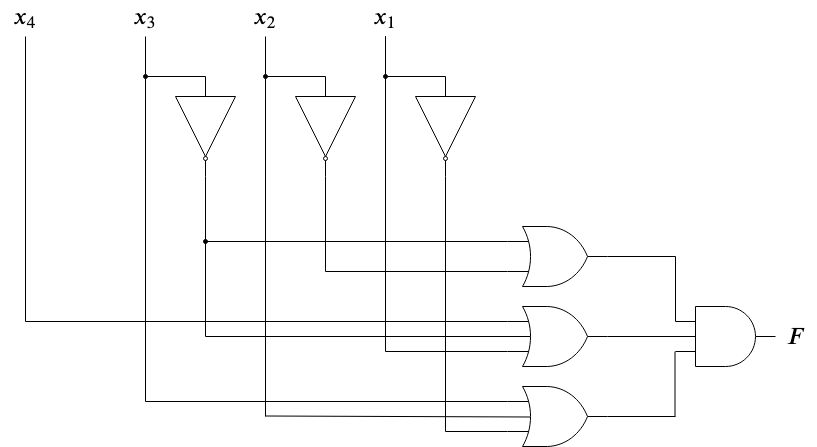
\includegraphics[width=15cm]{C3.jpg}
\end{center}
\caption{関数$F$に対するNOT-OR-AND形式の回路図}
\label{C3}
\end{figure}

\subsection*{D. 論理関数$F(x_4, x_3, x_2, x_1)$について、$F(0,0,0,1)=F(1,1,1,0)=F(0,0,1,1)=F(0,1,1,0)=F(1,1,0,0)=F(0,1,0,0)=F(1,1,0,1)=F(0,1,0,1)=1$、また、$F(0,1,1,1)=F(1,0,0,1)=F(1,0,1,1)=\ast$である。それ以外は$F=0$である。関数$F$を、Quine-McCluskey法を用いて簡単化し、そのNOT-AND-OR形式(積和標準形)の論理式を求めよ。}

まず、ドントケアを1と解釈し、極小項の統合を行う。統合を行った結果を図\ref{D0}に示す。ここで、$p$は肯定形変数の数であり、(a)から(c)の段階を経て統合される。この図でフラッグが立っていない項が主項である。

\begin{figure}[htbp]
	\begin{tabular}{ccc}
	\begin{minipage}{.33\textwidth}
		\centering
        \subcaption{(a)}
		\begin{tabular}{|c|ccccc|} \hline			
		$p = 1$ & 0 & 0 & 0 & 1 & \checkmark \\
        & 0 & 1 & 0 & 0 & \checkmark \\ \hline
        $p = 2$ & 0 & 0 & 1 & 1 & \checkmark \\
        & 0 & 1 & 0 & 1 & \checkmark \\
        & 0 & 1 & 1 & 0 & \checkmark \\
        & 1 & 0 & 0 & 1 & \checkmark \\
        & 1 & 1 & 0 & 0 & \checkmark \\ \hline
        $p = 3$ & 0 & 1 & 1 & 1 & \checkmark \\
        & 1 & 0 & 1 & 1 & \checkmark \\
        & 1 & 1 & 0 & 1 & \checkmark \\
        & 1 & 1 & 1 & 0 & \checkmark \\ \hline
		\end{tabular}
	\end{minipage}
	\begin{minipage}{.33\textwidth}
		\centering
        \subcaption{(b)}
		\begin{tabular}{|c|ccccc|} \hline			
		$p = 1$ & 0 & 0 & -- & 1 & \checkmark \\
        & 0 & -- & 0 & 1 & \checkmark \\
        & -- & 0 & 0 & 1 & \checkmark \\
        & 0 & 1 & 0 & -- & \checkmark \\
        & 0 & 1 & -- & 0 & \checkmark \\
        & -- & 1 & 0 & 0 & \checkmark \\ \hline
        $p = 2$ & 0 & -- & 1 & 1 & \checkmark \\
        & -- & 0 & 1 & 1 & \checkmark \\
        & 0 & 1 & -- & 0 & \checkmark \\
        & -- & 1 & 0 & 1 & \checkmark \\
        & 0 & 1 & 1 & -- & \checkmark \\
        & -- & 1 & 1 & 0 & \checkmark \\
        & 1 & 0 & -- & 1 & \checkmark \\
        & 1 & -- & 0 & 1 & \checkmark \\
        & 1 & 1 & 0 & -- & \checkmark \\
        & 1 & 1 & -- & 0 & \checkmark \\ \hline
		\end{tabular}
	\end{minipage}
	\begin{minipage}{.33\textwidth}
		\centering
        \subcaption{(c)}
		\begin{tabular}{|c|ccccc|} \hline			
		$p = 1$ & 0 & -- & -- & 1 &  \\
        & -- & 0 & -- & 1 &  \\
        & -- & -- & 0 & 1 &  \\
        & 0 & 1 & -- & -- &  \\
        & -- & 1 & -- & 0 &  \\
        & -- & 1 & 0 & -- &  \\ \hline
        \end{tabular}
	\end{minipage}
	\end{tabular}
    \caption {極小項のグループ分けと統合}
    \label{D0}
\end{figure}

次に、ドントケアを0と解釈し、関数値を1とする入力変数の値の組に対する極小項と主項に対して包含図を構成する。その結果が図\ref{D1}である。この包含図を2段階の手法で簡約化する。第1段階では、ある極小項を包含する主項が1つしかないものを使用が確定した基本主項とし、基本主項とその主項が包含する極小項を除外する。第1段階簡約化した結果が図\ref{D2}である。第2段階では、ある極小項を包含する主項がいずれも別の極小項を包含する場合、後者の極小項を除外する。第2段階簡約化した結果が図\ref{D3}である。


\begin{figure}
\begin{center}
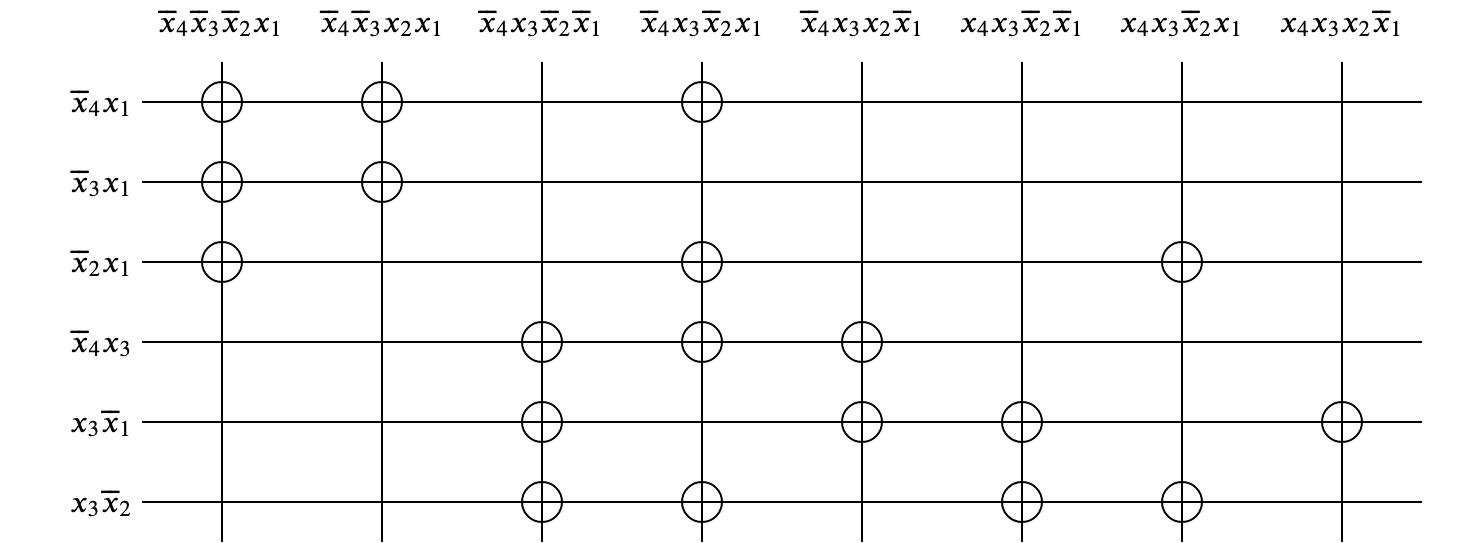
\includegraphics[width=15cm]{D1.jpg}
\end{center}
\caption{関数値1に対する極小項と主項の間の包含図}
\label{D1}
\end{figure}

\begin{figure}
\begin{center}
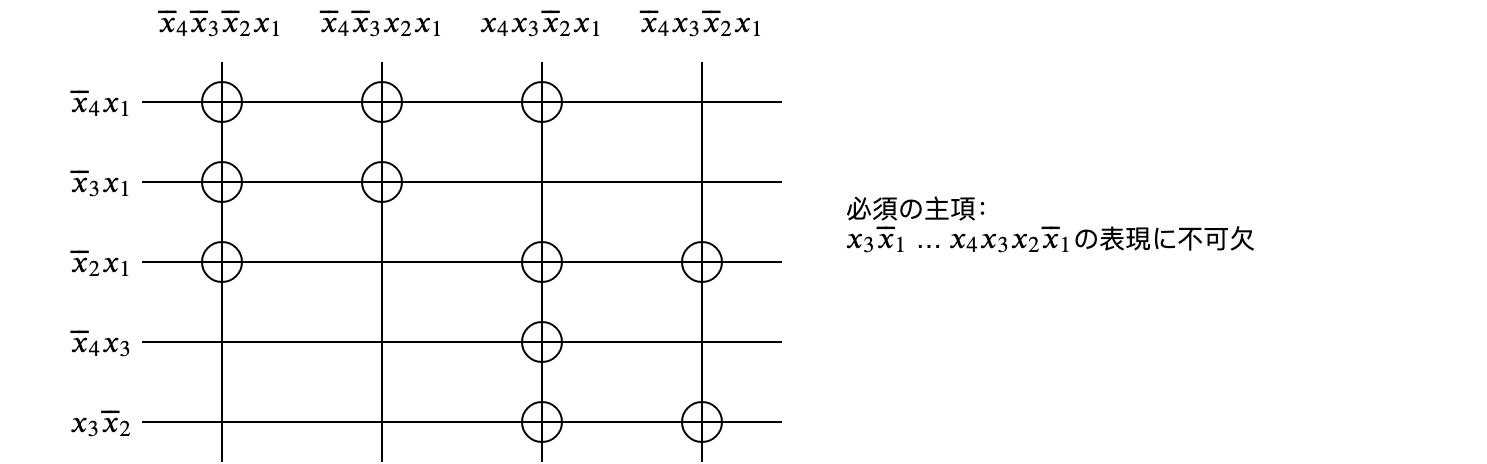
\includegraphics[width=15cm]{D2.jpg}
\end{center}
\caption{図\ref{D1}を第1段階簡約化したもの}
\label{D2}
\end{figure}

\begin{figure}
\begin{center}
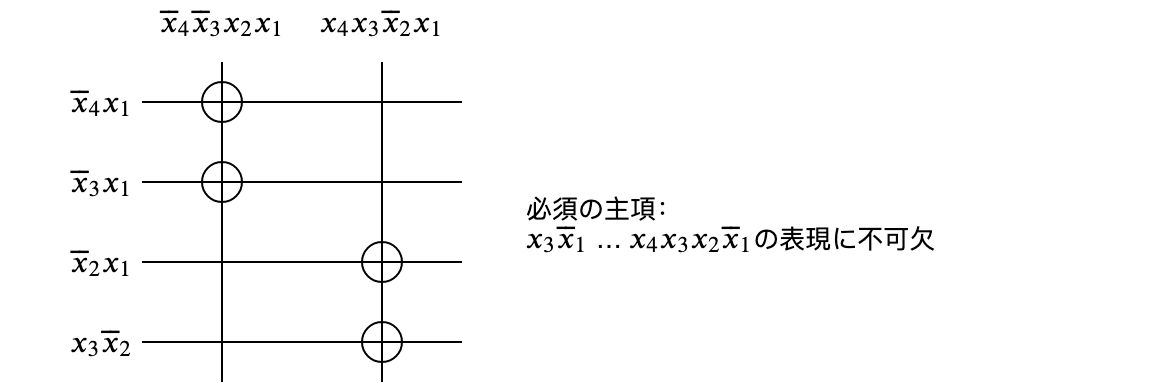
\includegraphics[width=12cm]{D3.jpg}
\end{center}
\caption{図\ref{D2}を第2段階簡約化したもの}
\label{D3}
\end{figure}

ここで、図\ref{D3}の極小項を表現するのに必要な主項について$A=\bar{x_4}x_1$、$B=\bar{x_3}x_1$、$C=\bar{x_2}x_1$、$D=x_3\bar{x_2}$とおくと、各極小項を表現しなければならないことを次の式で表せる。

\begin{eqnarray*}
(A \lor B)(C \lor D) = AC \lor AD \lor BC \lor BD
\end{eqnarray*}

以上より、第1段階で除外した基本主項をORで連結すると、論理関数$F(x_4, x_3, x_2, x_1)$を実現するNOT-AND-OR形式の論理式が以下のように複数得られる。

\begin{eqnarray*}
F(x_4, x_3, x_2, x_1) &=& \bar{x_4}x_1 \lor \bar{x_2}x_1 \lor x_3\bar{x_1} \\
&=& \bar{x_4}x_1 \lor x_3\bar{x_2} \lor x_3\bar{x_1} \\
&=& \bar{x_3}x_1 \lor \bar{x_2}x_1 \lor x_3\bar{x_1} \\
&=& \bar{x_3}x_1 \lor x_3\bar{x_2} \lor x_3\bar{x_1}
\end{eqnarray*}

これらの中で最も簡単なものを選ぶと、論理関数$F(x_4, x_3, x_2, x_1)$を簡単化した結果となる。

\begin{eqnarray*}
F(x_4, x_3, x_2, x_1) &=& \bar{x_3}x_1 \lor \bar{x_2}x_1 \lor x_3\bar{x_1} = \bar{x_3}x_1 \lor x_3\bar{x_2} \lor x_3\bar{x_1}
\end{eqnarray*}

\end{document}
